\documentclass[crop,tikz]{standalone}

\usetikzlibrary{calc}
\tikzset{>=latex}
\colorlet{green}{black!40!green}
\colorlet{gray}{gray!20}
\newcommand{\F}{\vec{F}}
\newcommand{\Z}{\vec{Z}}

\begin{document}
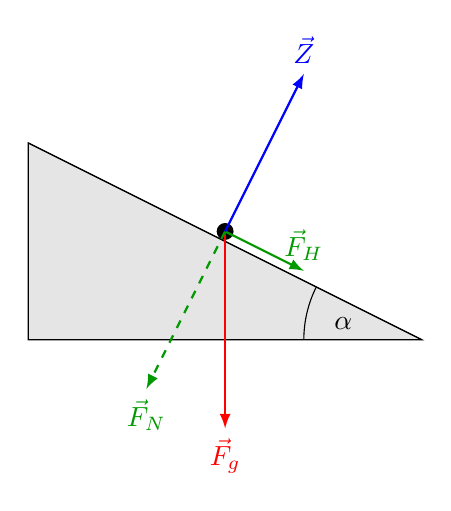
\begin{tikzpicture}[scale=2.5]
  \draw[fill=gray] (0,0) -- (2,0) -- (0,1) -- cycle;
  \draw (2,0) -- (0,1);
  \draw ([shift={(153.4:0.6)}]2,0) arc (153.4:180:0.6);
  \draw (1.6,0) node[above] {$\alpha$};
  \coordinate (a) at (1,0.55);
  \draw[fill,black] (a) circle (0.04);
  \draw[->,thick,red] (a) -- +(0,-1) node[below] {$\F_g$};
  \pgfmathsetmacro{\al}{atan(0.5)} % angle
  \pgfmathsetmacro{\sa}{sin(\al)}; % sin(angle)
  \pgfmathsetmacro{\ca}{cos(\al)}; % cos(angle)
  \draw[->,thick,green] (a) -- +($(\sa*\ca,-\sa*\sa)$) node[above] {$\F_H$};
  \draw[->,thick,green,dashed] (a) -- +($(-\sa*\ca,-\ca*\ca)$) node[below] {$\F_N$};
  \draw[->,thick,blue] (a) -- +($(\sa*\ca,\ca*\ca)$) node[above] {$\Z$};
\end{tikzpicture}
\end{document}
